%% The following is a directive for TeXShop to indicate the main file
%%!TEX root = diss.tex

\chapter{Background and Motivation}
\label{ch:BackgroundMotiv}

%%%%%%%%%%%%%%%%%%%%%%%%%%%%%%%%%%%%%%%%%%%%%%%%%%%%%%%%%%%%%%%%%%%%%%
%%
%% Opportunity
%%
%%%%%%%%%%%%%%%%%%%%%%%%%%%%%%%%%%%%%%%%%%%%%%%%%%%%%%%%%%%%%%%%%%%%%%

\section{Opportunity}
\label{sec:Opportunity}
\begin{figure}
    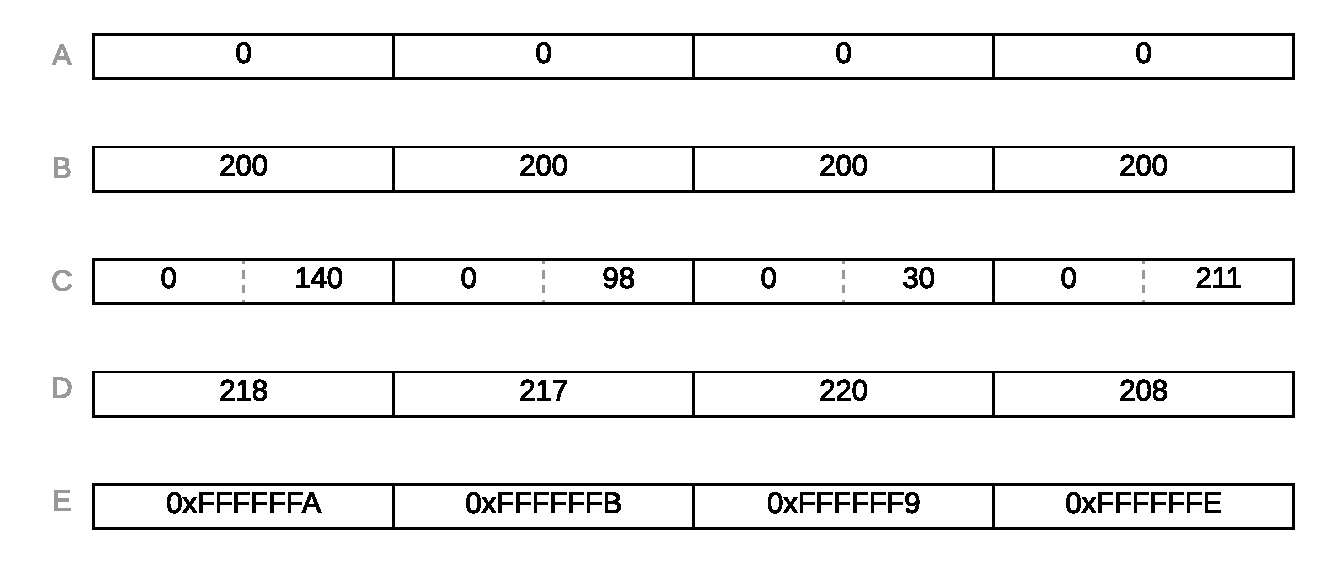
\includegraphics[width=\textwidth]{Patterns.pdf}
    \caption[Patterns in cache lines]{Some of the patterns observed in cache lines.}
    \label{fig:Patterns}
\end{figure}
\begin{figure}
    \begin{subfigure}[t]{\textwidth}
        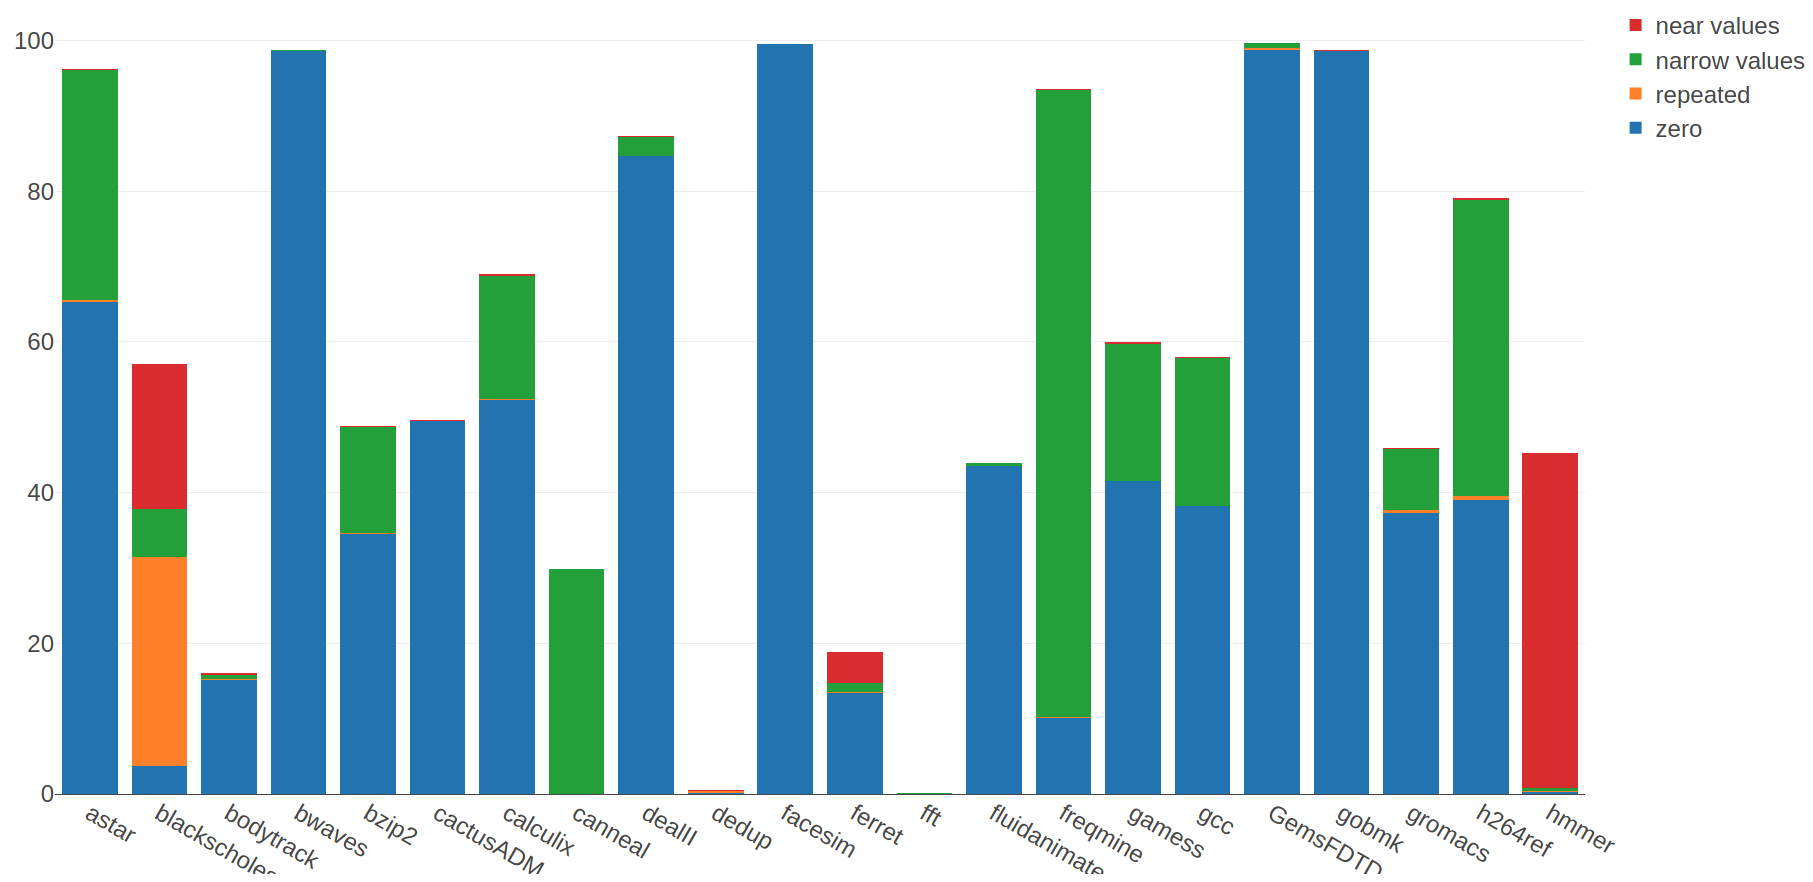
\includegraphics[width=\textwidth]{BDIPotential1.png}
    \end{subfigure}
    \begin{subfigure}[b]{\textwidth}
        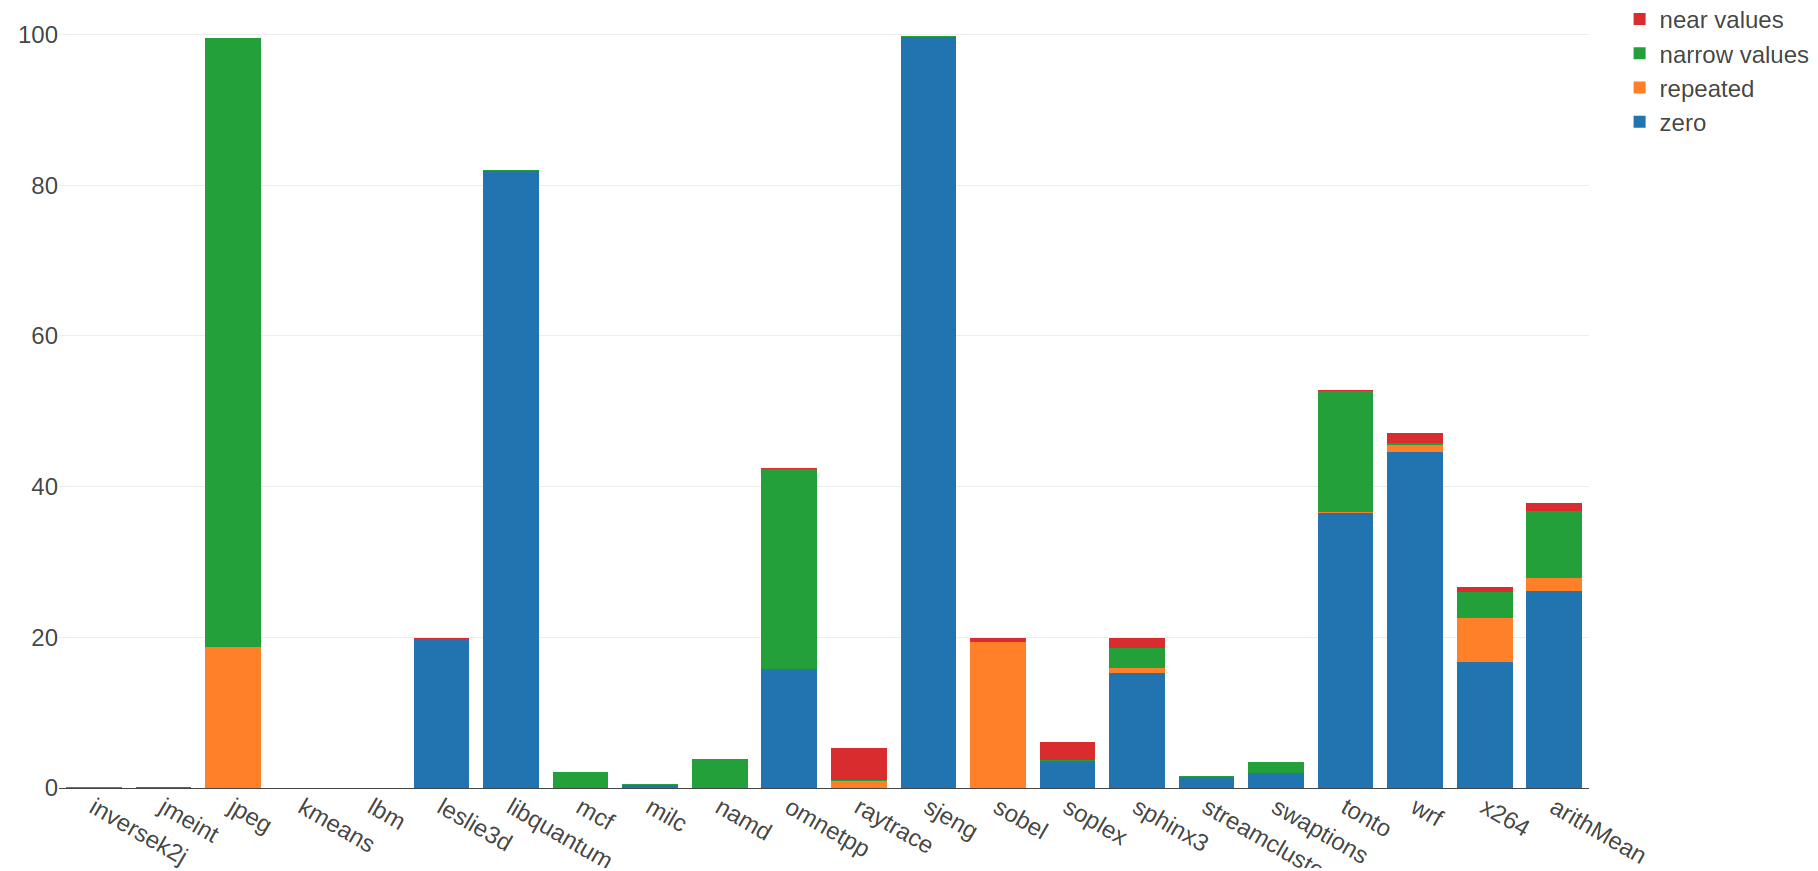
\includegraphics[width=\textwidth]{BDIPotential2.png}
    \end{subfigure}
    \caption[Intra-line Patterns]{The figure shows the percentage of cache lines that have one of the following patterns: zero, repeated values, narrow values, or near values. Recreated from \protect\cite{bdi}}
    \label{fig:BDIPotential}
\end{figure}
\begin{figure}
    \begin{subfigure}[t]{\textwidth}
        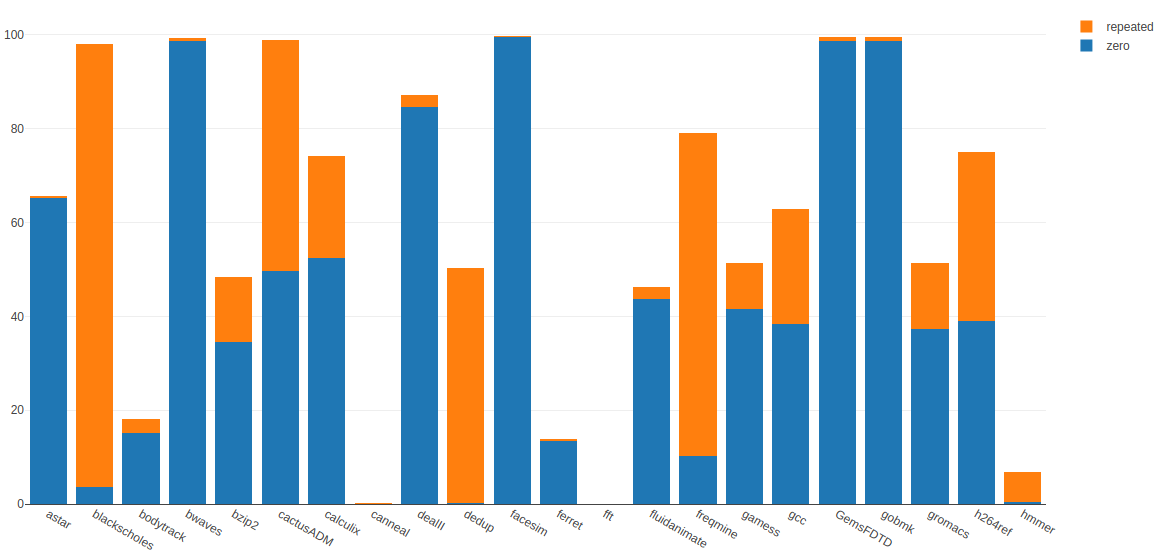
\includegraphics[width=\textwidth]{DedupPotential1.png}
    \end{subfigure}
    \begin{subfigure}[b]{\textwidth}
        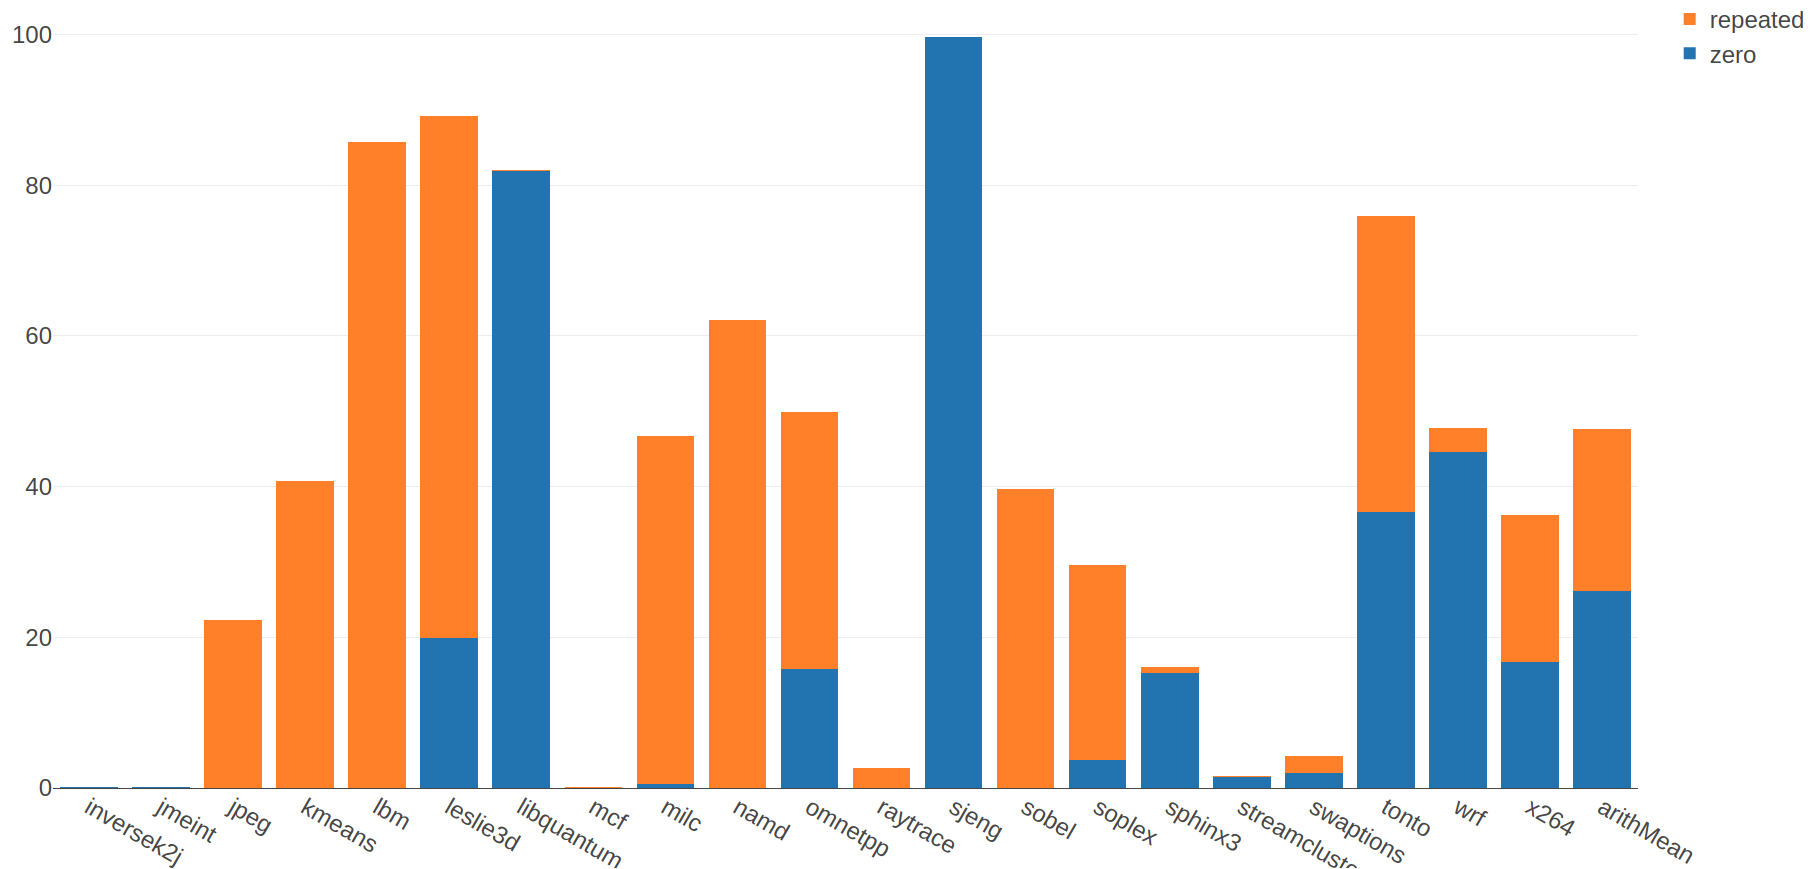
\includegraphics[width=\textwidth]{DedupPotential2.png}
    \end{subfigure}
    \caption[Inter-line Patterns]{The figure shows the percentage of similar cache lines in a cache, those present an opportunity for deduplication. Recreated from \protect\cite{dedup}}
    \label{fig:DedupPotential}
\end{figure}
Caches have been observed to have a great degree of redundancy when used with real world applications, those patterns can be observed on different granularities. We consider the patterns found on a cache line granularity, and on granularities smaller than a cache line. Some of those patterns are shown in Figure~\ref{fig:Patterns} and are described as follows:
\begin{enumerate}
    \item \textbf{intra-line granularity:}
    \begin{enumerate}
        \item \textbf{Zeros:} A lot of cache data lines are fully zeros~\cite{balakrishnan2003exploiting, ekman2005robust, yang2000frequent}. This is a very common case because zeros are usually used to initialize data structures. They're also very common in applications that deal with sparse matrices. Shown in part A of the figure.
        \item \textbf{Repeated Values:} Where a full cache line can contain the same value~\cite{sazeides1997predictability, alameldeen2004adaptive}. This can be observed in applications that initialize large arrays to the same initial value, or in multimedia applications where adjacent pixels could hold the same colours. Shown in part B of the figure.
        \item \textbf{Narrow Values:} Programmers typically code for the worst case and thus have to pick larger data types while the majority of the values can fit in smaller narrower data types~\cite{alameldeen2004adaptive, islam2010characterization, wilson1999case}. An example is a cache line of 32 bit integers where all the integer values are less than 256. A similar case is shown in part C of the figure.
        \item \textbf{Near Values:} Lines that contain values that are somewhat similar but not exactly, those are values that have high entropy in their lower bits but have the same higher bits. An example would be a list of pointers that are in the same memory regions, or pixels of an image that have almost similar colours~\cite{wilson1999case, sun2008dhtc}. Part D and E of the figure show examples of this case.
    \end{enumerate}
    \item \textbf{inter-line granularity:}
    \begin{enumerate}
        \item \textbf{Zero lines:} Similar to the first pattern in the previous point, this case is about data lines being fully zeros. The only difference here is that we consider different zero lines instead of one line being fully zeroed.
        \item \textbf{Repeated lines:} Multiple cache lines can be exactly the same. This can happen in scientific benchmarks that have symmetry~\cite{dedup}. For example the benchmark bwaves~\cite{spec} simulates a spherical blast wave around an origin point, which involves perfect similarities.
    \end{enumerate}
\end{enumerate}
Figures~\ref{fig:BDIPotential} and~\ref{fig:DedupPotential} show the percentage of cache lines where those inter-line and intra-line patterns occur. A modified version of the zsim~\cite{zsim} simulator have been used to dump snapshots of the L3 cache every 100,000 L3 accesses, with a maximum of 10 dumps per benchmark. The figures were created by statically analyzing the dumps for patterns.

%%%%%%%%%%%%%%%%%%%%%%%%%%%%%%%%%%%%%%%%%%%%%%%%%%%%%%%%%%%%%%%%%%%%%%
%%
%% BDI Cache
%%
%%%%%%%%%%%%%%%%%%%%%%%%%%%%%%%%%%%%%%%%%%%%%%%%%%%%%%%%%%%%%%%%%%%%%%

\section{Intra-line Compression}
\label{sec:BDI}
The BDI cache introduced in~\cite{bdi} is a cache that takes advantage of similarities within data lines to compress those lines into smaller sizes. In the following section we discuss the BDI cache, its compression, structure, and operation.
\subsection{Compression}
\label{Compression}
\subsubsection{Base Delta Compression}
In the previously mentioned patterns, the data in a cache line granularity have a low dynamic range, the difference between values in one cache line can be represented using fewer bytes than the original data type. A compression scheme was proposed to utilize this low dynamic range. It works by representing the data line using a base value, and an array of delta values. Since the delta values can be smaller in size than the original data elements, this allows for a lot of savings in the data line itself. If the delta size required to represent the delta is not smaller than the original size, the line is then not compressible and is left untouched.\par
Finding the right base is key to compress the data line optimally, and it happens in two steps:
\begin{itemize}
    \item \textbf{Finding the base size:} The right base size would affect the deltas and their sizes, and thus will affect the final compression size. Since caches have no knowledge of the data types stored in them, compression is not able to identify whether a specific data line is comprised of 16 bit integers or 32 bit floats and so the base size is not directly known. Choosing one base size statically would greatly reduce the opportunity for compression, so the authors opted to allow three different base sizes: 2, 4 and 8 bytes that can used simultaneously and the one that provides the best compression should be used.
    \item \textbf{Finding the base value:} Once a base size is chosen, the base value itself mush be found. Ideally, selecting the base value in a compressed line should be in the middle point between the minimum and the maximum values of a cache line. To avoid the hardware implementation complexity of finding the base, the authors opted to use the first value as base.
\end{itemize}
The allowed compression schemes and compressed sizes are shown in Figure~\ref{fig:BaseDeltaCompression} and table~\ref{tab:BDICompressionSizes}.
\begin{figure}
    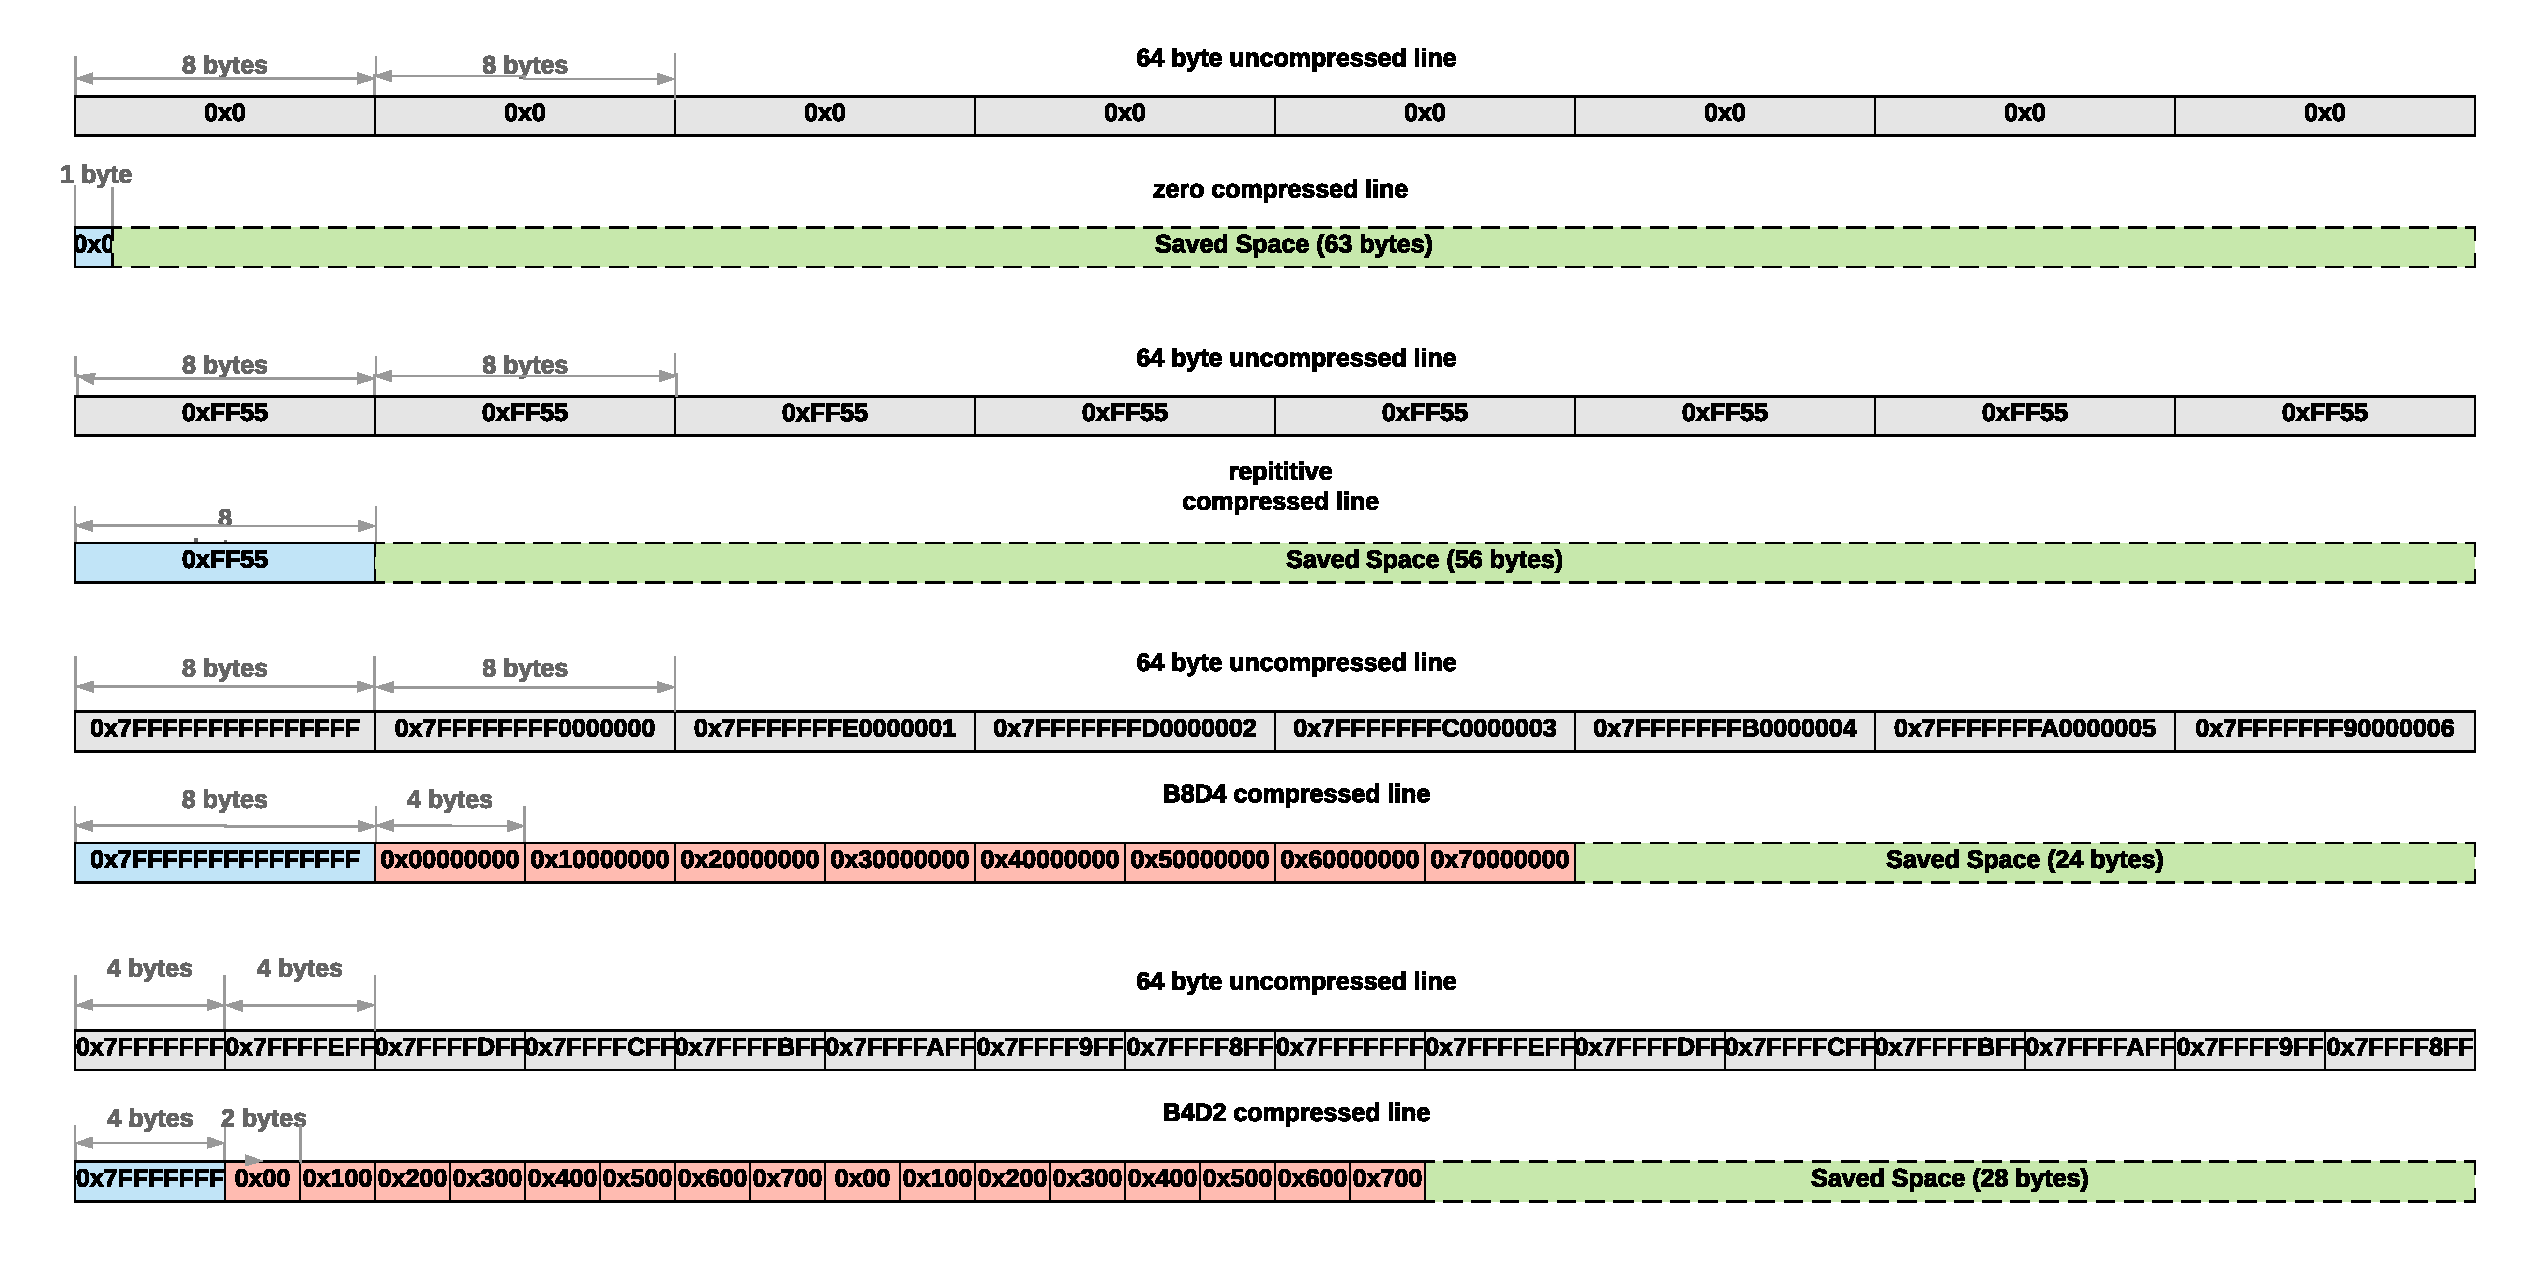
\includegraphics[width=\textwidth]{BaseDeltaCompression.pdf}
    \caption[Base Delta Compression Examples]{The figure shows examples of different cases of Base Delta compression.}
    \label{fig:BaseDeltaCompression}
\end{figure}
\subsubsection{Base Delta Immediate Compression}
Although one can gain a lot of compression from the base delta compression scheme, some patterns cannot be represented just by one base value. An example would be applications that use structs comprising of different data types. Because of this, allowing the base delta compression to use more than one base might help compress such lines. Based on experiments in~\cite{bdi} it was clear that bases more than two do not provide much compression, so the authors selected two bases as their optimum number. To avoid the complexity of looking for a second base when compressing a data line, the authors opted to use the second base as an implicit zero. The intuition behind this is when structs are used in applications, they're likely to contain wide values with low dynamic range (e.g. Pointers) along with narrow values, the authors observe that using an implicit zero base captures most of the compression enabled by using an arbitrary second base.
\begin{table}[]
\centering
\caption[BDI Sizes]{The table shows BDI compression sizes, all sizes are in bytes. Original line size is 64 bytes.}
\label{tab:BDICompressionSizes}
\begin{tabular}{|c|c|c|c|c|}
\hline
\textbf{Name}         & \textbf{\begin{tabular}[c]{@{}c@{}}Base\\ Size\end{tabular}} & \textbf{\begin{tabular}[c]{@{}c@{}}Delta\\ Size\end{tabular}} & \textbf{\begin{tabular}[c]{@{}c@{}}Compression\\ Size\end{tabular}} & \textbf{\begin{tabular}[c]{@{}c@{}}Compression\\ Encoding\end{tabular}} \\ \hline
\textbf{Zero}         & 1                                                            & 0                                                             & 1                                                                   & 0000                                                                    \\ \hline
\textbf{Rep}          & 8                                                            & 0                                                             & 8                                                                   & 0001                                                                    \\ \hline
\textbf{B8D1}         & 8                                                            & 1                                                             & 16                                                                  & 0010                                                                    \\ \hline
\textbf{B8D2}         & 8                                                            & 2                                                             & 24                                                                  & 0011                                                                    \\ \hline
\textbf{B8D4}         & 8                                                            & 4                                                             & 40                                                                  & 0100                                                                    \\ \hline
\textbf{B4D1}         & 4                                                            & 1                                                             & 20                                                                  & 0101                                                                    \\ \hline
\textbf{B4D2}         & 4                                                            & 2                                                             & 36                                                                  & 0110                                                                    \\ \hline
\textbf{B2D1}         & 2                                                            & 1                                                             & 34                                                                  & 0111                                                                    \\ \hline
\textbf{Uncompressed} & N/A                                                          & N/A                                                           & 64                                                                  & 1111                                                                    \\ \hline
\end{tabular}
\end{table}
\subsubsection{Compression Hardware}
\label{sssec:BDICompressionHardware}
The compression hardware used for BDI consists of eight units that operate simultaneously in parallel, two for the zero and repetitive compression schemes and six units for the three different bases with their deltas. Each unit corresponds for one of the compression sizes described in Table~\ref{tab:BDICompressionSizes}. Each unit outputs whether the line can be compressed in its scheme or not, and if it can be compressed it also outputs the compressed line. If multiple units can compress the line then the selection logic picks the one with the least compressed size.
A compression unit treats the line as elements of its corresponding base size. It picks the first element as the base and then subtracts all the elements from the it. If all the results can be represented in the required delta size then the line is compressed. Figure~\ref{fig:BDIHardware} shows the compression hardware.
\begin{figure}
    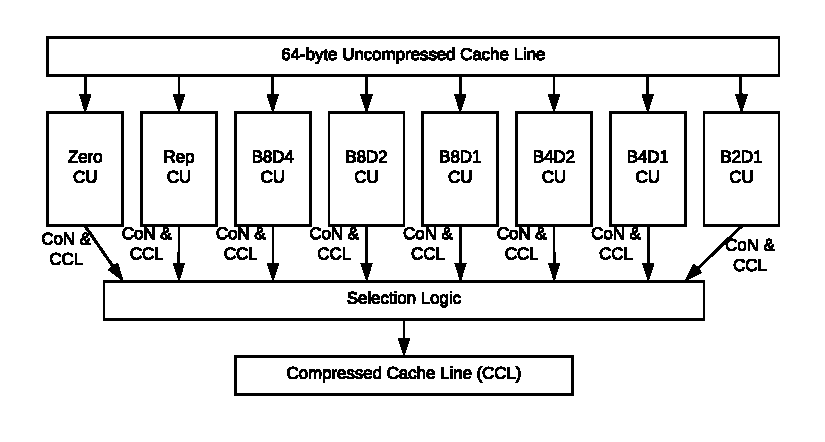
\includegraphics[width=\textwidth]{BDIHardware.pdf}
    \caption[BDI Compression Hardware]{The figure shows BDI compression hardware. CU: Compression Unit, CoN: Compressed or Not?, CCL: Compressed Cache Line. Recreated from \protect\cite{bdi}}
    \label{fig:BDIHardware}
\end{figure}

\subsection{Structure}
\label{ssec:BDIStructure}
\begin{figure}
    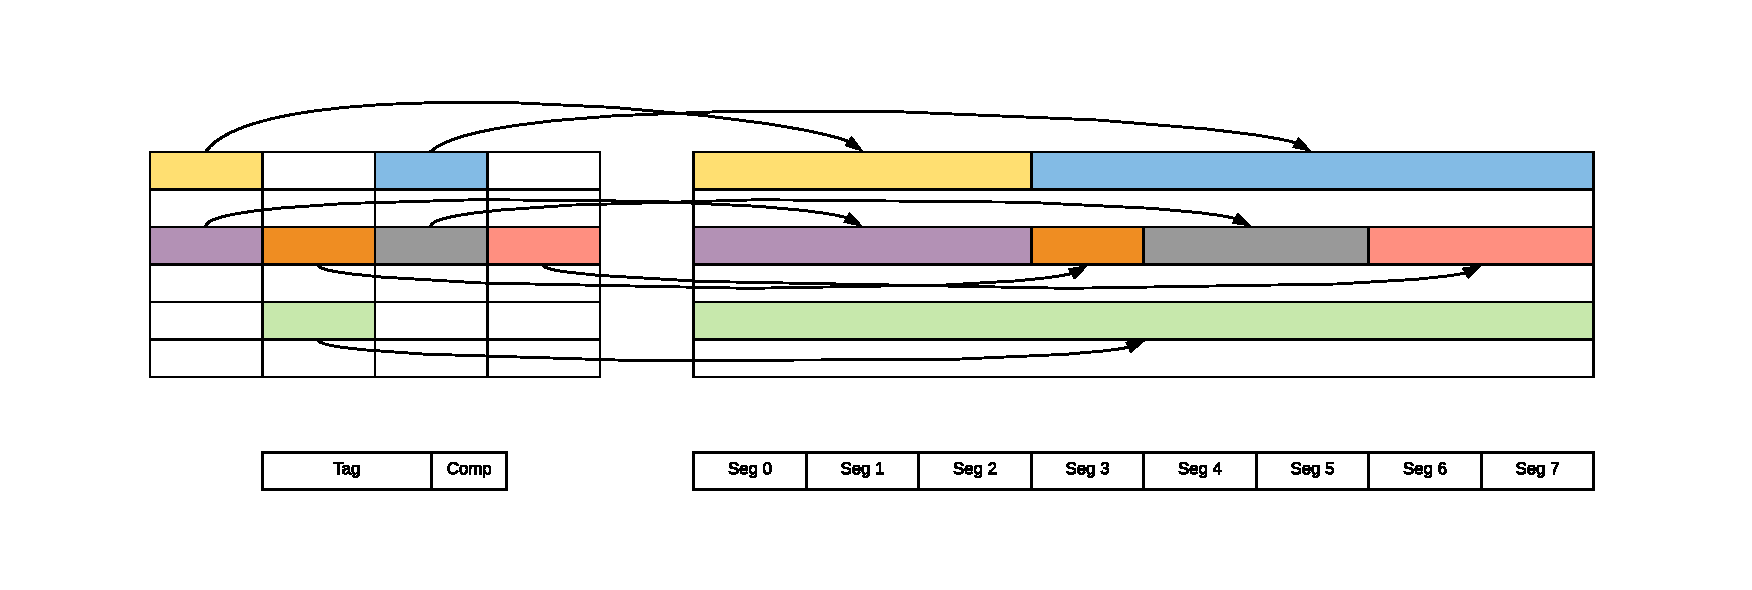
\includegraphics[width=\textwidth]{BDI.pdf}
    \caption[BDI Cache]{Conventional (up) vs BDI (down), showing one set of each. Tags doubled, Data size same but divided to segments.}
    \label{fig:BDI}
\end{figure}
The BDI cache builds upon the conventional cache design by adding some modifications to allow compression. Tag and data arrays are arranged in sets, and tag sets and data sets are coupled. The BDI cache structure is shown in Figure~\ref{fig:BDI}
\subsubsection{Tag Array}
\label{sssec:BDITag}
Tag arrays in a BDI cache are no different than their counterparts in a conventional cache. The tags are arranged in sets and ways.\par
Along with its normal function, the tags also have two extra fields: A compression metadata field, and a Segment pointer. The compression metadata field describes the type of compression in the corresponding data line, it also contains a mask to distinguish which base is used for each delta. The segment pointer field is used to point to the first segment of the corresponding data line.\par
Other than the addition of compression metadata and segment pointer no other changes happen to the tag array. There are no constraint on its organization or replacement policy. However, because BDI potentially allows more data to be stored in the same cache size, more tags are needed to address this data. The tag array has to generally have more tags than data lines otherwise no benefits come out of compression.
\subsubsection{Data Array}
\label{sssec:BDIData}
Data lines in a BDI cache are logically divided into eight fixed size segments of eight bytes each (assuming a 64 byte cache line). A compressed data line can occupy any number of segments between one and eight. The data array does not save any metadata.\par
This general structure means the cache no longer has coupled tag and data \textit{lines} but it still maintains coupled data and tag \textit{sets}, i.e. A tag entry is no longer associated with a data entry in the corresponding location in the data array, but is associated with one of the segments in the corresponding set in the data array. The location of that segment depends on the compression encodings in the current selected tag set.

\subsection{Operations}
\label{ssec:BDIOperations}
\begin{figure}[h]
    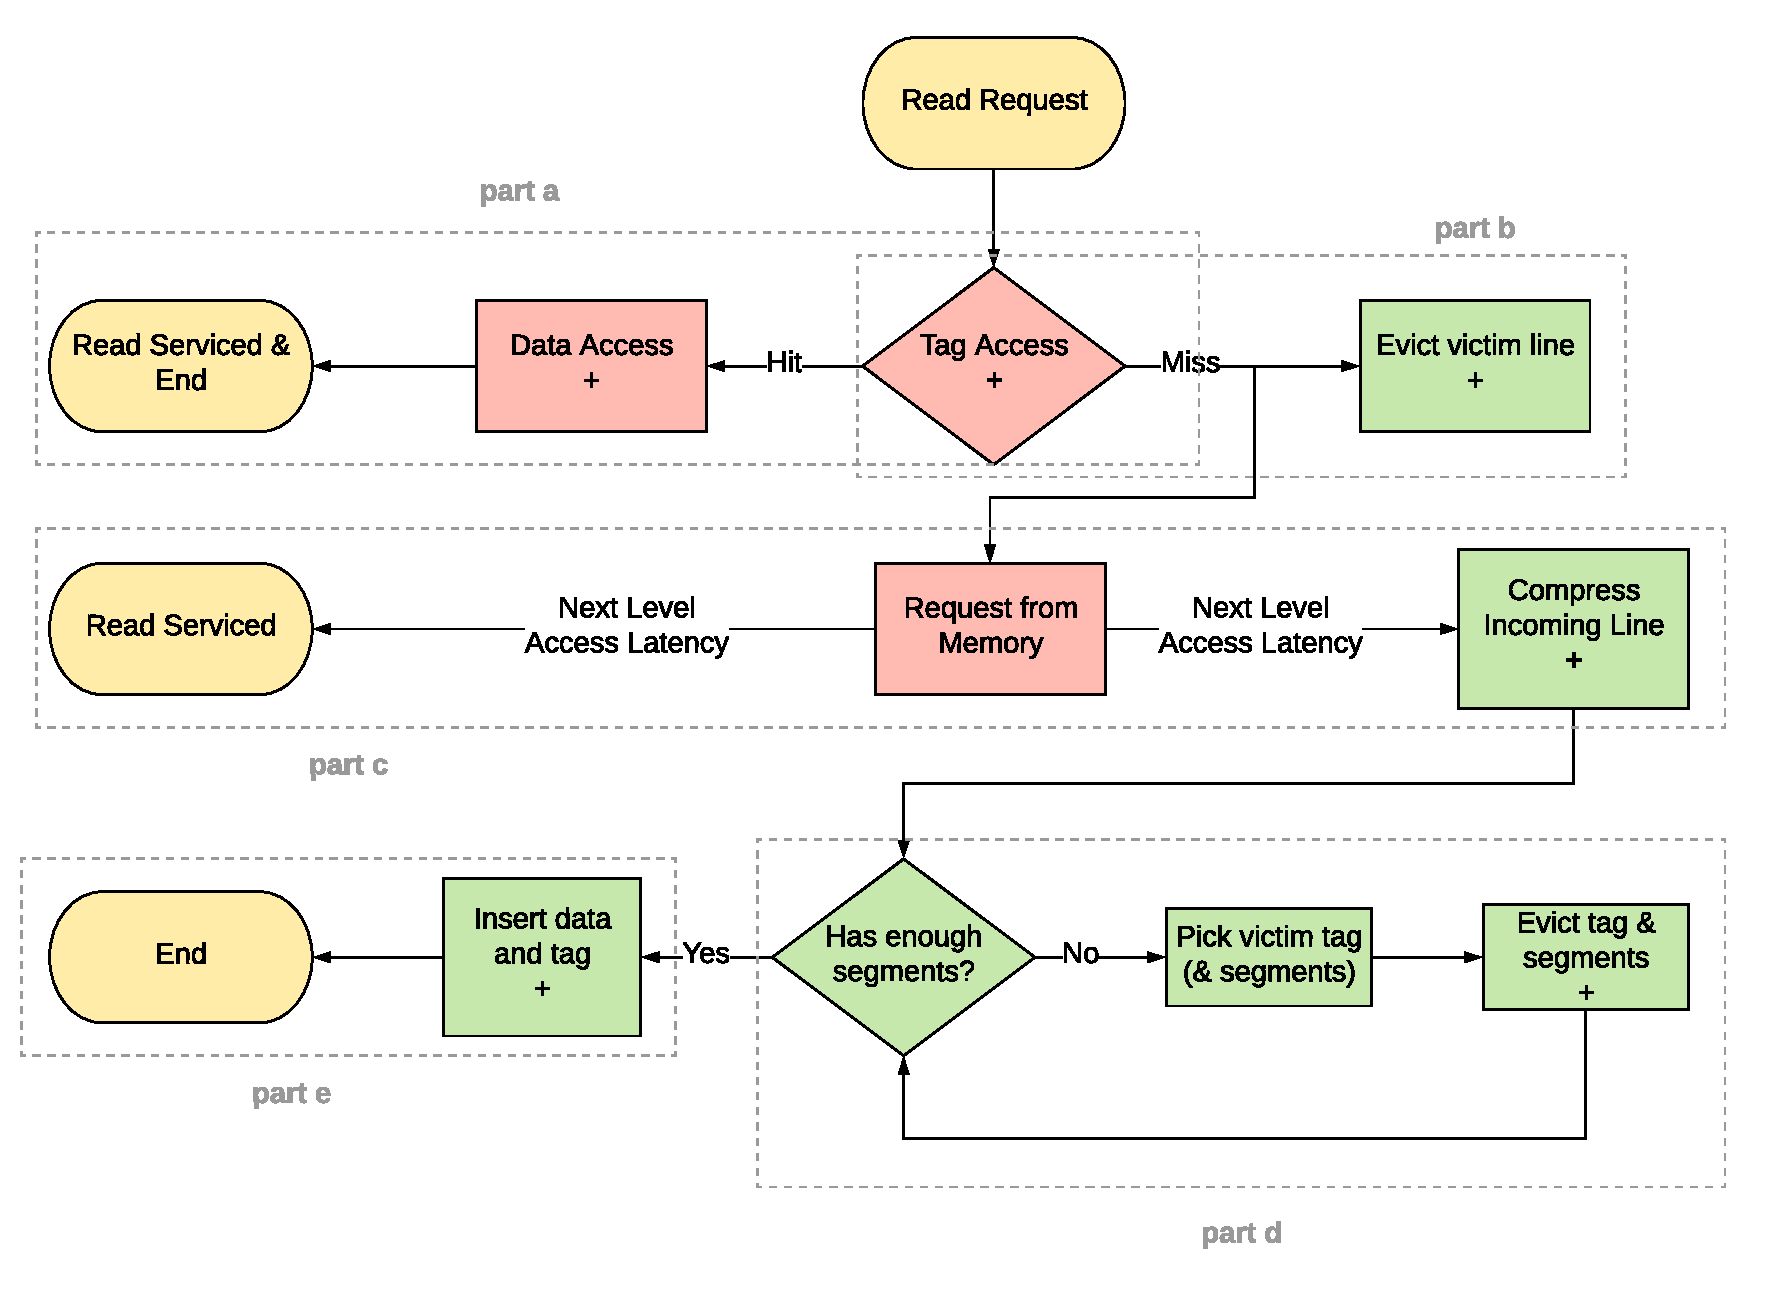
\includegraphics[width=\textwidth]{BDI_Read.pdf}
    \caption[BDI Read]{The flowchart shows the sequence of actions triggered by a read access to the BDI cache. Red blocks signify actions happening on the critical path, while green blocks mean actions happening off the critical path. Each + sign in any of the blocks signifies an extra latency for tag array access, data array access, or compression.}
    \label{fig:BDI_Read}
\end{figure}
\subsubsection{Cache Read}
A flowchart for the BDI cache read is shown in Figure~\ref{fig:BDI_Read}. When the request first arrives the tag array is accessed. Part a in the figure shows the case when the tag access results in a hit, then the data line can be read, decompressed, and sent back to the requester right away. If the tag access is a miss, as shown in part b, the victim line is evicted. Then at the same time in parallel a request is sent to the next cache level (or main memory). Once the requested line comes back from the next level it can be used to service the requester right away, inserting the line itself into the cache happens after that and off the critical path, as shown in part c.\par
So far through the access everything is similar to a conventional cache, Only the insertion of the new line is going to be different. The insertion of the new line starts in part c in the figure. Once the requested line comes back from next level, and in parallel to serving the requester, the line is BDI compressed. Then before the line is actually written to the cache we must verify that there is enough space in the data set for it. If there's not enough segments we have to trigger extra evictions in the current set to free up more segments, those evictions happen according to the tag replacement policy. The size caused evictions are shown in part d, and the line can finally be inserted once enough segments are available as shown in part e.\par
To avoid segmentation, the authors assume compaction always happens in the data array before each insertion, this is in accordance with previous work.
\begin{figure}[h]
    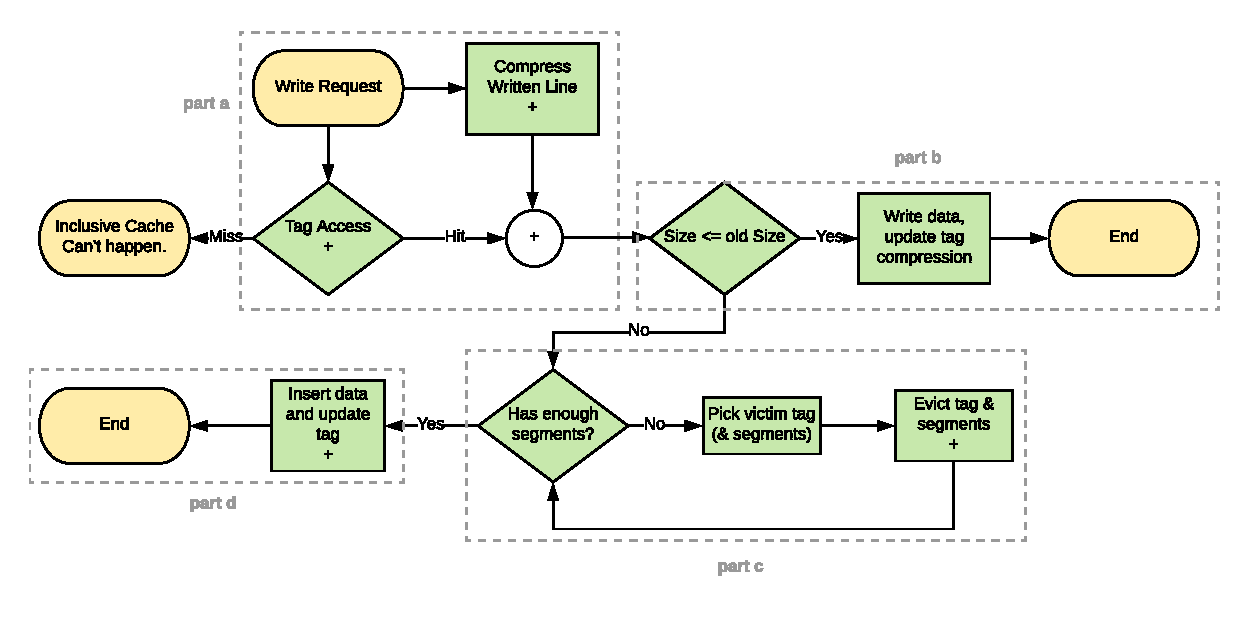
\includegraphics[width=\textwidth]{BDI_Write.pdf}
    \caption[BDI Write]{The flowchart shows the sequence of actions triggered by a write access to the BDI cache. All the blocks are shaded in green because any write request should be off the critical path of the processor regardless of its status in the cache (hit or miss). Each + sign in any of the blocks signifies an extra latency for tag array access, data array access, or compression.}
    \label{fig:BDI_Write}
\end{figure}
\subsubsection{Cache Write}
A flowchart of write access to a BDI cache is shown in Figure~\ref{fig:BDI_Write}. Because we always use inclusive caches, if a line is in a lower level cache it must also be in its parent. A cache miss on a write request thus can never happen and a tag array access on a write request will always yield a hit as shown in part a. In parallel to the tag access, the written data line can also be compressed. Once we know the size of the compressed line, we can check whether or not it fits in its old size, if it is the same or requires a lower number of segments, shown in part b, it can be written right away and the compression metadata in the tag array must also be updated. If the new compressed size is bigger than the old size, insertion of the new written line will trigger size based evictions, the replacement policy will be consulted for tags and their segments to be evicted until enough space for the new data line is free, this is shown in part c. Once there's enough segments the line can finally be written and its tag's metadata can be updated accordingly as shown in part d.
As mentioned previously, the authors assume compaction always happens in the data array before each insertion, this is in accordance with previous work.

%%%%%%%%%%%%%%%%%%%%%%%%%%%%%%%%%%%%%%%%%%%%%%%%%%%%%%%%%%%%%%%%%%%%%%
%%
%% Dedup Cache
%%
%%%%%%%%%%%%%%%%%%%%%%%%%%%%%%%%%%%%%%%%%%%%%%%%%%%%%%%%%%%%%%%%%%%%%%
\section{Inter-line Compression}
\label{sec:Dedup}
The Dedup cache was introduced in~\cite{dedup}. The authors have found that in some applications, a lot of lines in the cache can be similar, as shown in Figure~\ref{fig:DedupPotential}. Previous cache compression implementations have been proposed to take advantage of duplications, but only focused on special cases like zeros~\cite{alameldeen2004adaptive, dusser2009zero}. The authors proposed and built a cache that takes full advantage of the line similarity by doing deduplication, getting rid of the redundant data copies and keeping only one. The structure and operation of such a cache is discussed in this section.
\subsection{Structure}
\label{ssec:DedupStructure}
\begin{figure}
    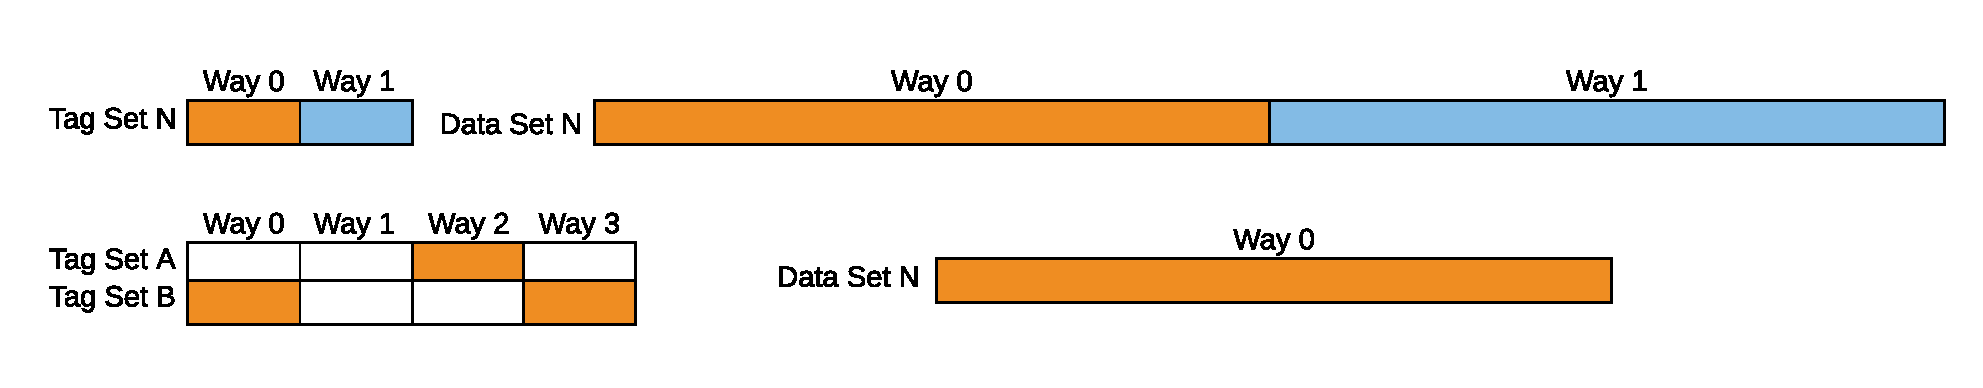
\includegraphics[width=\textwidth]{Dedup.pdf}
    \caption[Dedup Cache]{Conventional (up) vs Dedup (down), showing one set of tags and data from a conventional cache, but one set and related tags from a dedup cache. Tags doubled, Data size same but is now direct mapped.}
    \label{fig:Dedup}
\end{figure}
The Dedup cache introduces some major modifications on top of a conventional cache to support deduplication. The tag array is arranged as normal in sets and ways. The data array is no longer coupled with the tag array, instead it has to be explicitly accessed by pointers. So the data array has no constraints or requirements on its associativity, so it is simply left to be direct mapped. To take advantage of deduplications, the tag array must generally have more entries than the data array.\par
To facilitate finding and locating duplicate lines, a new structure is added to the cache, called the hash array. The hash array is a storage that saves hashes of data lines. Searching and comparing in the hash array makes it faster and cheaper than searching for duplicate lines directly in the data cache.

The Dedup cache structure is shown in Figure~\ref{fig:BDI}

\subsubsection{Tag Array}
\label{sssec:DedupTag}
The Dedup tag array organization is no different than a tag array in a conventional cache, it is arranged in sets and ways.\par
To support deduplication, some other modifications to the tag array need to be made. Deduplication means more than one tag entry will share the same data entry. This poses two requirements on the Dedup cache: Tags must know which data line is the one they need, and if that data line gets evicted, all the tags that use it must be evicted too.\par
based on the previous requirements, some additions to the tag array entries must be made. For the tags to be able to address their corresponding data lines, a pointer to the data line must be added to the tag entry. Similarly, to facilitate eviction of all the tags connected to a data line when the line is evicted, those tags are organized in a linked list, so each tag entry has two previous and next pointers that point to the two tags before and after it in a linked list. Those pointers need to be big enough to only point to tag sets, since reading a tag requires reading the whole set, the required tag from that set can be resolved by comparing its data pointer.\par
Other than the addition of the previous/next and data pointers, there are no other changes to the tag array, only that tags need to have more entries than data to take advantage of deduplication.
\subsubsection{Data Array}
\label{sssec:DedupData}
The data array in a Dedup cache is decoupled from the tag array, and thus it is not required to have the same associativity as the tag array. In fact, this means the data array is not required to have any associativity at all, it can be directly mapped.\par
To facilitate the eviction of the tags associated with the data line in case it gets evicted, the data lines have an extra metadata field, a tag pointer. This tag pointer is used to point to the first tag in the linked list associated with the data line, in case the data line is evicted the linked list is walked and all the tags in it are evicted.\par
The data line also includes an extra counter, this counter is used to track how many tags use this data line, this is useful to decide which data lines to evict.
\subsubsection{Hash Array}
\label{sssec:DedupHash}
The hash array in a Dedup cache is used to store hashes of some of the data lines, providing a way to facilitate finding similar lines and deduplicating them. The hash array is a simple set associative structure.\par
When a data line is hashed, its hash is split into two parts, one is used to index the hash array, while the other is saved in the hash array itself. This process is similar to how memory addresses access the tag array, where part of the address is used to index the array while the other part is saved in the array itself.\par
Along with each hash saved in the hash array, there's also a pointer to a data line that meets this hash, similar to the data pointers in tag arrays.\par
The hashes are computed through an XOR tree, based on experiments done in~\cite{dedup}. The number of hash entries in the array is small. The authors in~\cite{dedup} show that a small number of hash entries is enough to keep collisions less that 1\%.

\subsection{Replacement Policies}
\label{ssec:DedupRepl}
While the tag array in a Dedup cache maintains its normal replacement policies, the data and hash array may have to be treated differently, since they're decoupled from the tag array.
\subsubsection{Data Array}
\label{sssec:DedupDataRepl}
The data array replacement policy can be split into two parts, the first part is uses a list to keep track of all free lines in the data array, this list is always consulted first for a free line to insert into. If the free list is empty, indicating that there are no free lines in the data array, the second part of the replacement policy is then used.\par
If no free lines are available, a random data line is selected, if that line is distinct (not deduplicated, has one tag), it is evicted and used for insertions, otherwise another random line is selected. This process is repeated up to four times, if after those four times no distinct line has been found, the line with the lowest deduplications is evicted and used for insertion.
\subsubsection{Hash Array}
\label{sssec:DedupHashRepl}
The hash array is indexed by a part of the hash, the selection of a victim hash set is thus dependant on the hash that needs to be inserted. Once that set is selected, a hash entry is then selected based on the number of deduplication on the data line it point to, if this data line is not deduplicated then this hash can be used and overwritten, otherwise it is not touched. The rationale behind this is to keep hashes pointing to deduplciated lines from getting evicted and causing the cache to miss extra deduplication in favour of a newly incoming line that might not be useful for deduplication.\par

\subsection{Operations}
\label{ssec:DedupOperations}
\begin{figure}[h]
    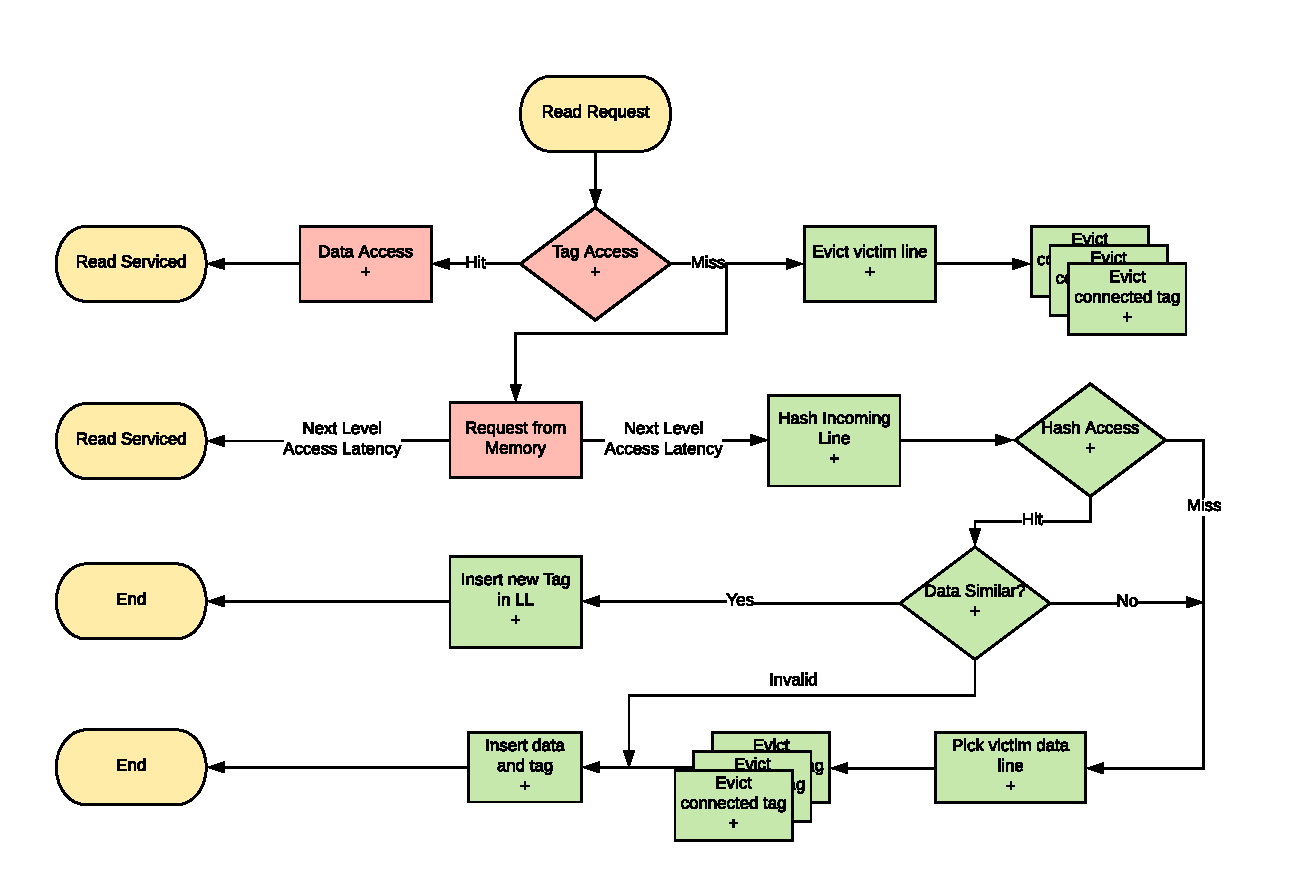
\includegraphics[width=\textwidth]{Dedup_Read.pdf}
    \caption[Dedup Read]{The flowchart shows the sequence of actions triggered by a read access to the Dedup cache. Red blocks signify actions happening on the critical path, while green blocks mean actions happening off the critical path. Each + sign in any of the blocks signifies an extra latency for tag array access, data array access, or compression.}
    \label{fig:Dedup_Read}
\end{figure}
\subsubsection{Cache Read}
A flowchart for the Dedup cache read is shown in Figure~\ref{fig:Dedup_Read}. When the request first arrives the tag array is accessed. Part a in the figure shows the case when the tag access results in a hit, then the data line can be read and sent back to the requester right away. If the tag access is a miss, as shown in part b, a victim tag is evicted and its linked list (if any) has to be updated (i.e. The pointers of the previous and next tags have to connect to each other instead of the victim.). At the same time and in parallel a request is sent to the next cache level (or main memory). Once the requested line comes back from the next level it can be used to service the requester right away, as shown in part c. Inserting the line itself into the cache happens after that and off the critical path.\par
So far through the access everything is similar to a conventional cache, Only the insertion of the new line is going to be different. The insertion of the new line starts in part d in the figure. Once the requested line comes back from next level, and in parallel to serving the requester, the line is hashed and the hash is used to access the hash array.\par
If the hash access hits, then the incoming line must be compared to the line pointed to by the hash, to make sure there are not collisions. There are four outcomes of this scenario, shown in part d:
\begin{itemize}
    \item \textbf{Hash Miss:} No similar hash is found, either because similar lines do not exist in the data array, or because the hash array is not big enough to keep track of all data lines. In this case we use the data replacement policy to evict a victim data line. The new tag is inserted and the tag and data lines have to point to each other, the tag will not point to other tags and will not create a linked list because no deduplication is happening yet. A new hash entry will be selected based on the hash replacement policy and will point to the newly inserted data line.
    \item \textbf{Hash Hit, Line Similar:} In which case the received data line can be deduplicated. It will use the same data line and hash entry. Only the new tag needs to be inserted. It is inserted as the head of the linked list and points to the deduplicated data line. The data line's tag counter (deduplication counter) has to be incremented and it has to point to the new linked list head.
    \item \textbf{Hash Hit, Line Invalid:} Because hashes point to data lines, but data lines do not point to hashes, when a data line is evicted, its associated hash might not, causing a situation like this to arise. In this case, we utilize the invalid line right away instead of consulting the data replacement policy. The tag entry is inserted, it has to point to the data line, but it doesn't point to any other tags because the data line is not deduplicated yet and shouldn't have a linked list associated with it. The data line in return also points to the tag entry, the hash entry is not changed because it already points to the space we used for the data line.
    \item \textbf{Hash Hit, Line Different:} This case happens only on a hash collision, when two different data lines can be hashed to the same value. Once a collision happens, it is treated like a hash miss with one modification: a new hash insertion is not needed. The same hash entry will be changed to point to the newly inserted data line in only if the line it was previously pointing to was not deduplicated (i.e. Its tag counter is 1). Otherwise it remains untouched.
\end{itemize}

\begin{figure}[h]
    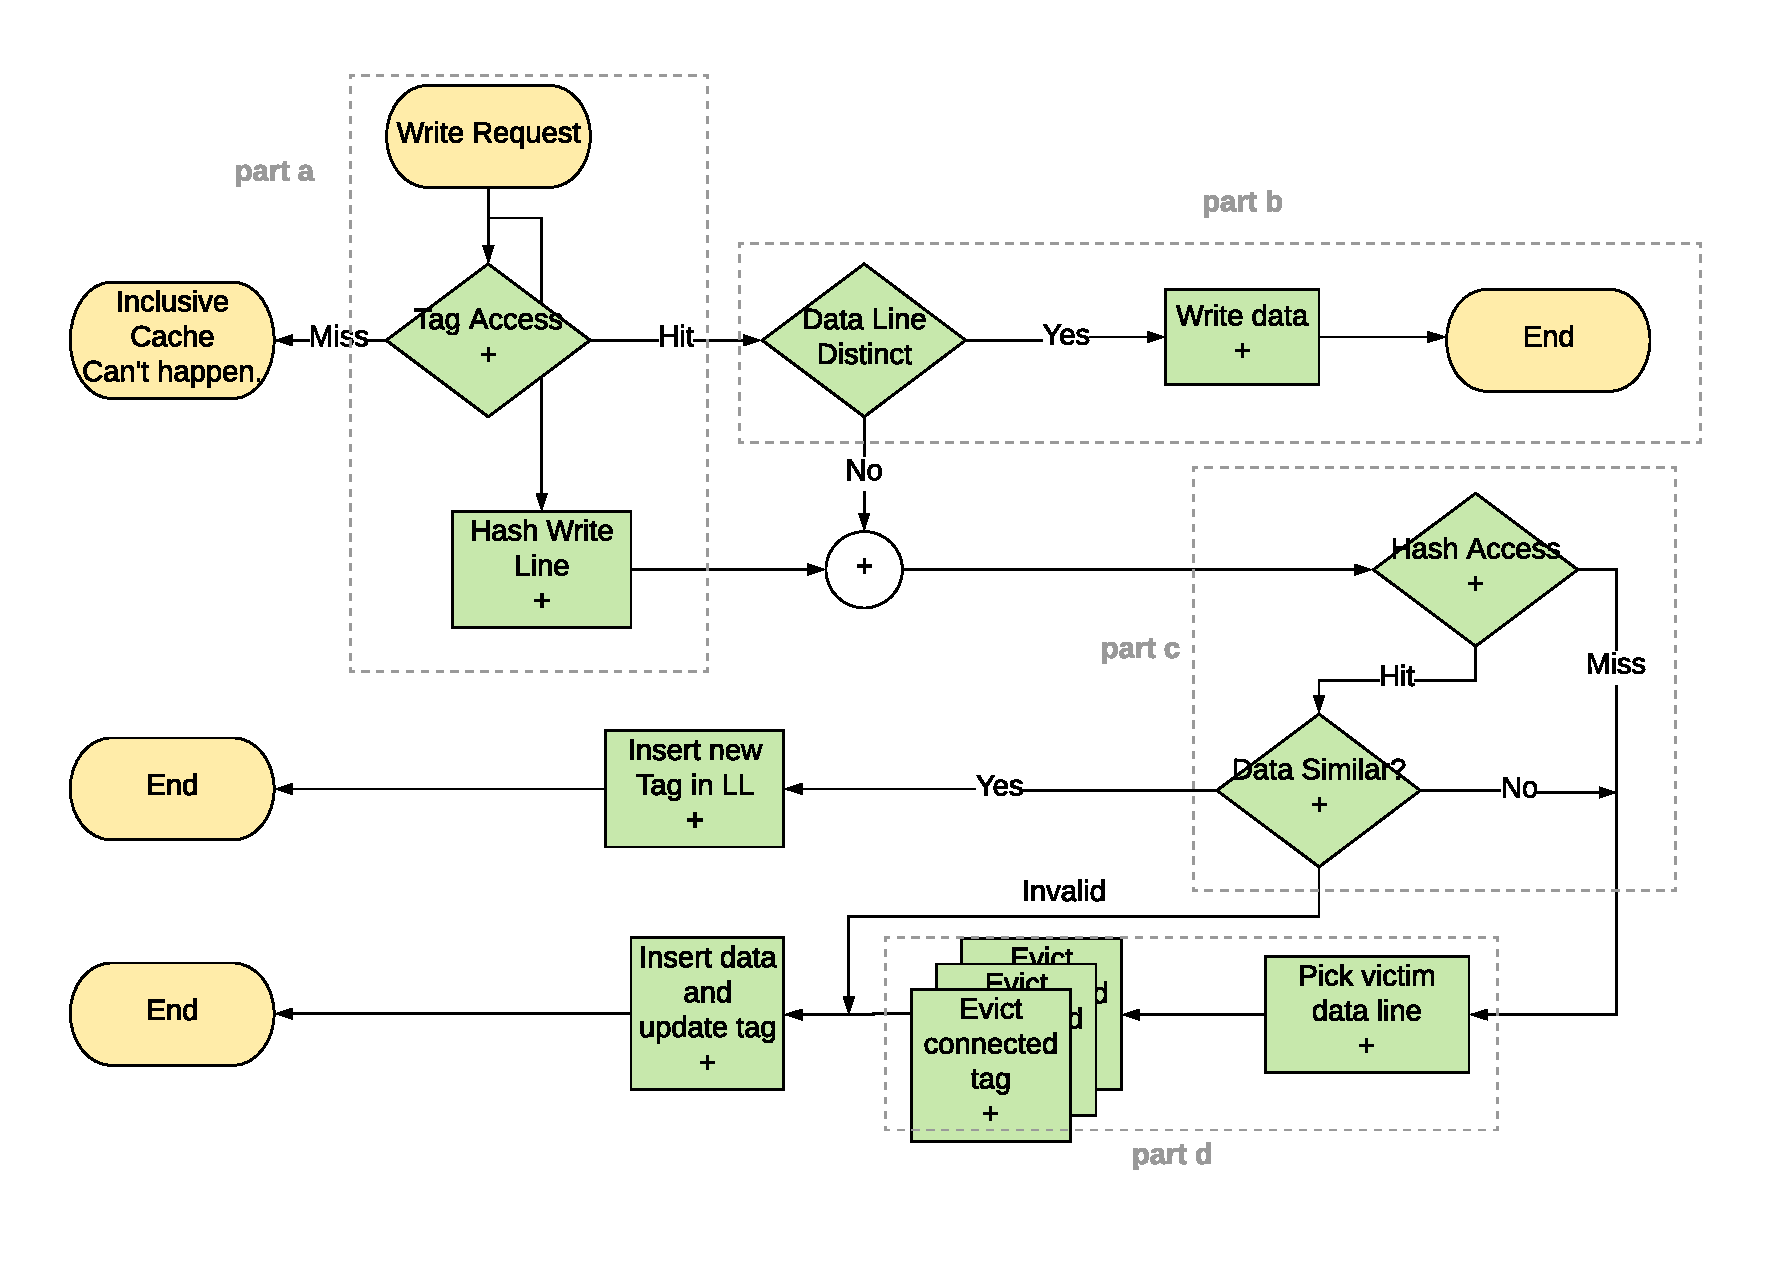
\includegraphics[width=\textwidth]{Dedup_Write.pdf}
    \caption[Dedup Write]{The flowchart shows the sequence of actions triggered by a write access to the Dedup cache. All the blocks are shaded in green because any write request should be off the critical path of the processor regardless of its status in the cache (hit or miss). Each + sign in any of the blocks signifies an extra latency for tag array access, data array access, or compression.}
    \label{fig:Dedup_Write}
\end{figure}
\subsubsection{Cache Write}
A flowchart of write access to a Dedup cache is shown in Figure~\ref{fig:Dedup_Write}. Because we always use inclusive caches, if a line is in a lower level cache it must also be in its parent. A cache miss on a write request thus can never happen and a tag array access on a write request will always yield a hit as shown in part a. In parallel to the tag access, the written data line can also be hashed.\par
Once the tag access is finished, we can find out whether the line was distinct or not. If the line is distinct and had no other tags associated with it, then it can be written to right away as shown in part b. If the line is deduplicated, then a write to the line can change it and cause that tag to lose similarity. The insertion of the written data line then can be handled similarly to a miss. It has to access the hash array and look for similar lines, this has one of the four outcomes described above as shown in parts c and d.

\section{Motivation}
\label{sec:Motivation}
Deduplication and base delta immediate compression work on two different domains, one is inter-line and works on a cache line granularity while the other works intra-line with a granularity of two, four, or eight bytes. This means that they can both be combined to deduplicate similar lines and compress each of those lines at the same time.
We look at four different benchmarks with different cache patterns and behaviors. One benchmark is very compressible by BDI, the second is compressible using deduplication, the third and fourth are completely incompressible and compressible by both, respectively. We analyze how these benchmarks respond to each type of compression and how a combination of both compression techniques can improve on them.\par
The four benchmarks are:
\begin{figure}
    \begin{subfigure}{0.5\textwidth}
        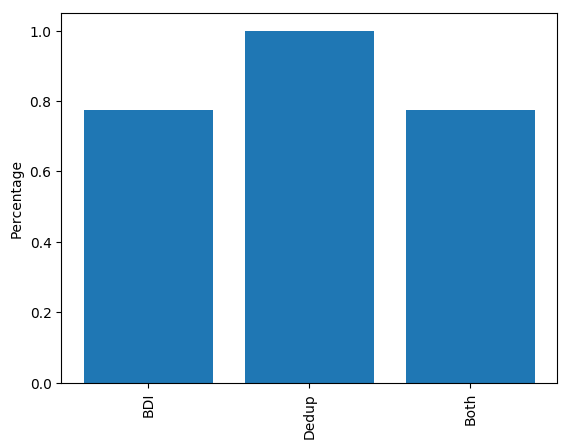
\includegraphics[width=\textwidth]{canneal.png}
        \caption{canneal}
        \label{fig:canneal}
    \end{subfigure}
    \begin{subfigure}{0.5\textwidth}
        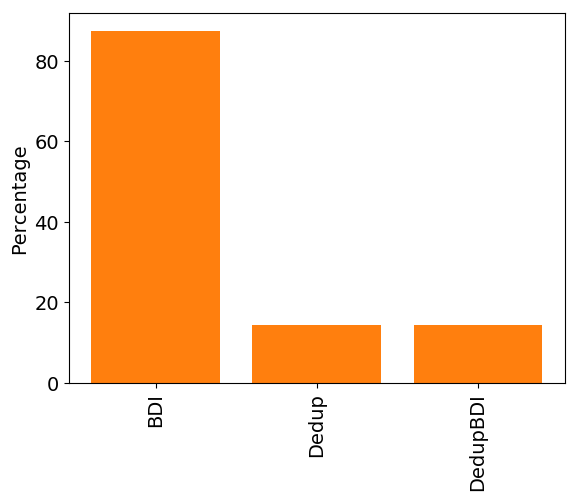
\includegraphics[width=\textwidth]{lbm.png}
        \caption{lbm}
        \label{fig:lbm}
    \end{subfigure}
    \begin{subfigure}{0.5\textwidth}
        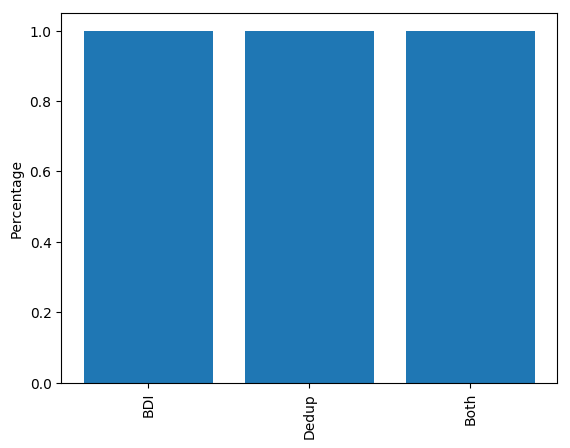
\includegraphics[width=\textwidth]{jmeint.png}
        \caption{jmeint}
        \label{fig:jmeint}
    \end{subfigure}
    \begin{subfigure}{0.5\textwidth}
        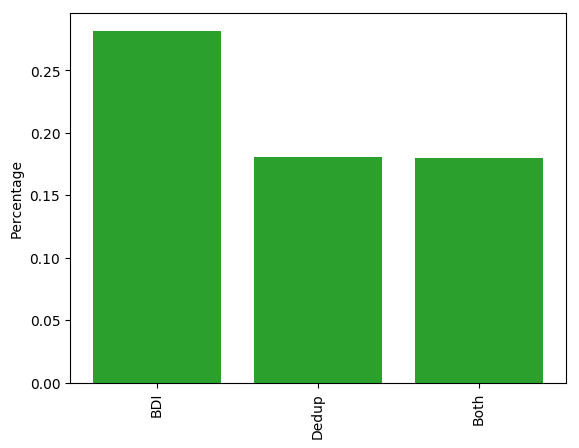
\includegraphics[width=\textwidth]{libquantum.png}
        \caption{libquantum}
        \label{fig:libquantum}
    \end{subfigure}
    \caption[Compression in benchmarks]{The figure shows the percentage of compressed data compared to original cache sizes.}
\end{figure}
\begin{itemize}
    \item \textbf{canneal:} The canneal benchmark~\cite{parsec} is a cache-aware implementation of a simulated annealing algorithm used for routing in chip designs. canneal is BDI sensitive but doesn't have enough potential to benifit from deudplication. Figure~\ref{fig:canneal} shows the Dedup, BDI, and Dedup+BDI compressed data size of canneal cache dumps as a percentage of the original size.
    \item \textbf{lbm:} The lbm benchmark~\cite{spec} implements the "Lattice Boltzman Method" to simulate incompressible fluids in 3D. The output from lbm benchmark is values representing 3d velocity vectors for each cell in the simulation. Because of this, lbm is deduplication sensitive. Figure~\ref{fig:lbm} shows the Dedup, BDI, and Dedup+BDI compressed data size of lbm cache dumps as a percentage of the original size.
    \item \textbf{jmeint:} The jmeint benchmark~\cite{axbench} is a triangle intersection workload that is used in 3d gaming. It takes coordinates of two triangles as its input. This makes most of the data insensitive to BDI compression and deduplication. Figure~\ref{fig:jmeint} shows the Dedup, BDI, and Dedup+BDI compressed data size of jmeint cache dumps as a percentage of the original size.
    \item \textbf{libquantum:} The libquantum library~\cite{spec} is used to simulate quantum computers. Specifically it simulates the Shor factorization algorithm widely used for cryptanalysis. It contains (at least at the first few cache dumps) a lot of zero lines which are 2D compressible through deduplication and BDI. Figure~\ref{fig:libquantum} shows the Dedup, BDI, and Dedup+BDI compressed data size of libquantum cache dumps as a percentage of the original size.
\end{itemize}
\begin{figure}
    \begin{subfigure}[t]{\textwidth}
        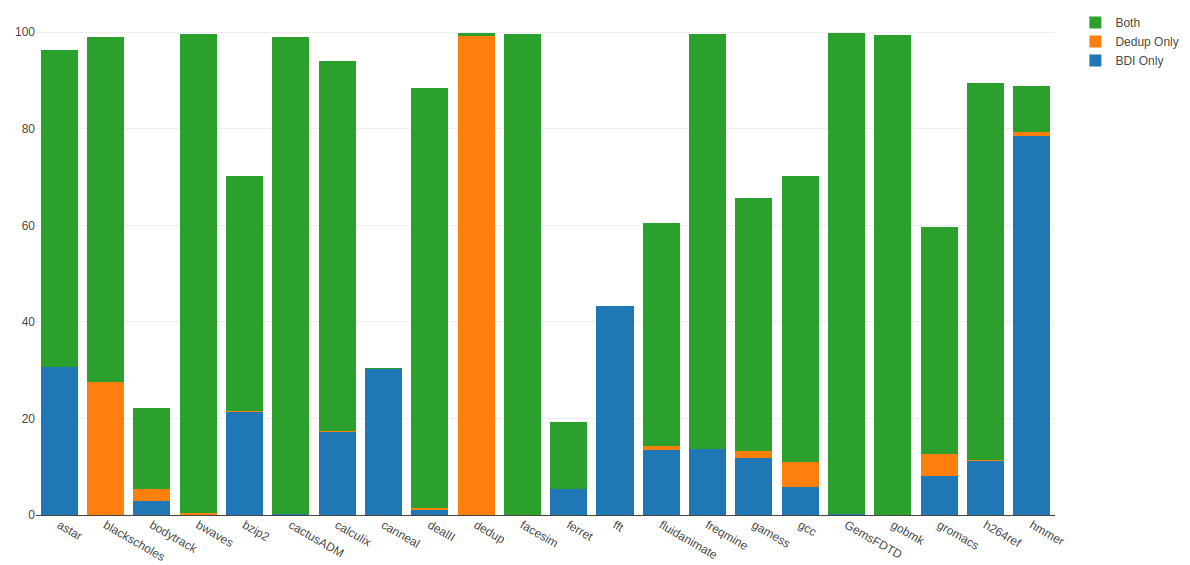
\includegraphics[width=\textwidth]{CompPotential1.png}
    \end{subfigure}
    \begin{subfigure}[b]{\textwidth}
        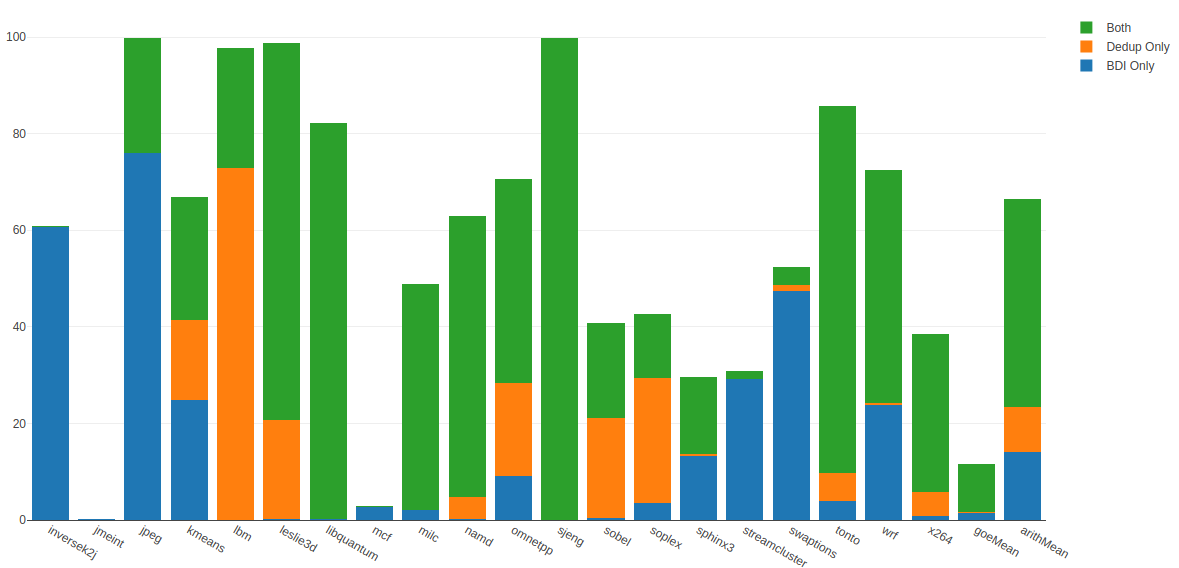
\includegraphics[width=\textwidth]{CompPotential2.png}
    \end{subfigure}
    \caption[Compressible lines]{The figure shows the percentage of cache lines that can be compressed using Dedup, BDI, or both techniques combined together.}
    \label{fig:CompPossibility}
\end{figure}
Generalizing on what we found. We used the same cache dumps to create Figure~\ref{fig:CompPossibility} showing the percentage of cache lines that can be compressed by BDI, the percentage of cache lines that are similar and thus deduplicable, and the percentage of cache lines that can be compressed using both schemes.\par
As Figure~\ref{fig:CompPossibility} shows, BDI and Deduplications are orthogonal to some degree. The existence of some cache lines that can be compressed by only one of both compression schemes means they can work separately without affecting each other. However, because there are lines that can be compressed by both schemes, BDI can lose some of its improvements because of deduplication. For example, if ten lines were similar and compressible by BDI, using BDI will compress each of them on its own, using deduplication will reduce all ten lines to only one line. Using both techniques means deduplication still compresses ten lines to one, but BDI now compresses only one line instead of 10. The improvements of BDI can thus be limited by deduplication.\par
\begin{figure}
    \begin{subfigure}[t]{\textwidth}
        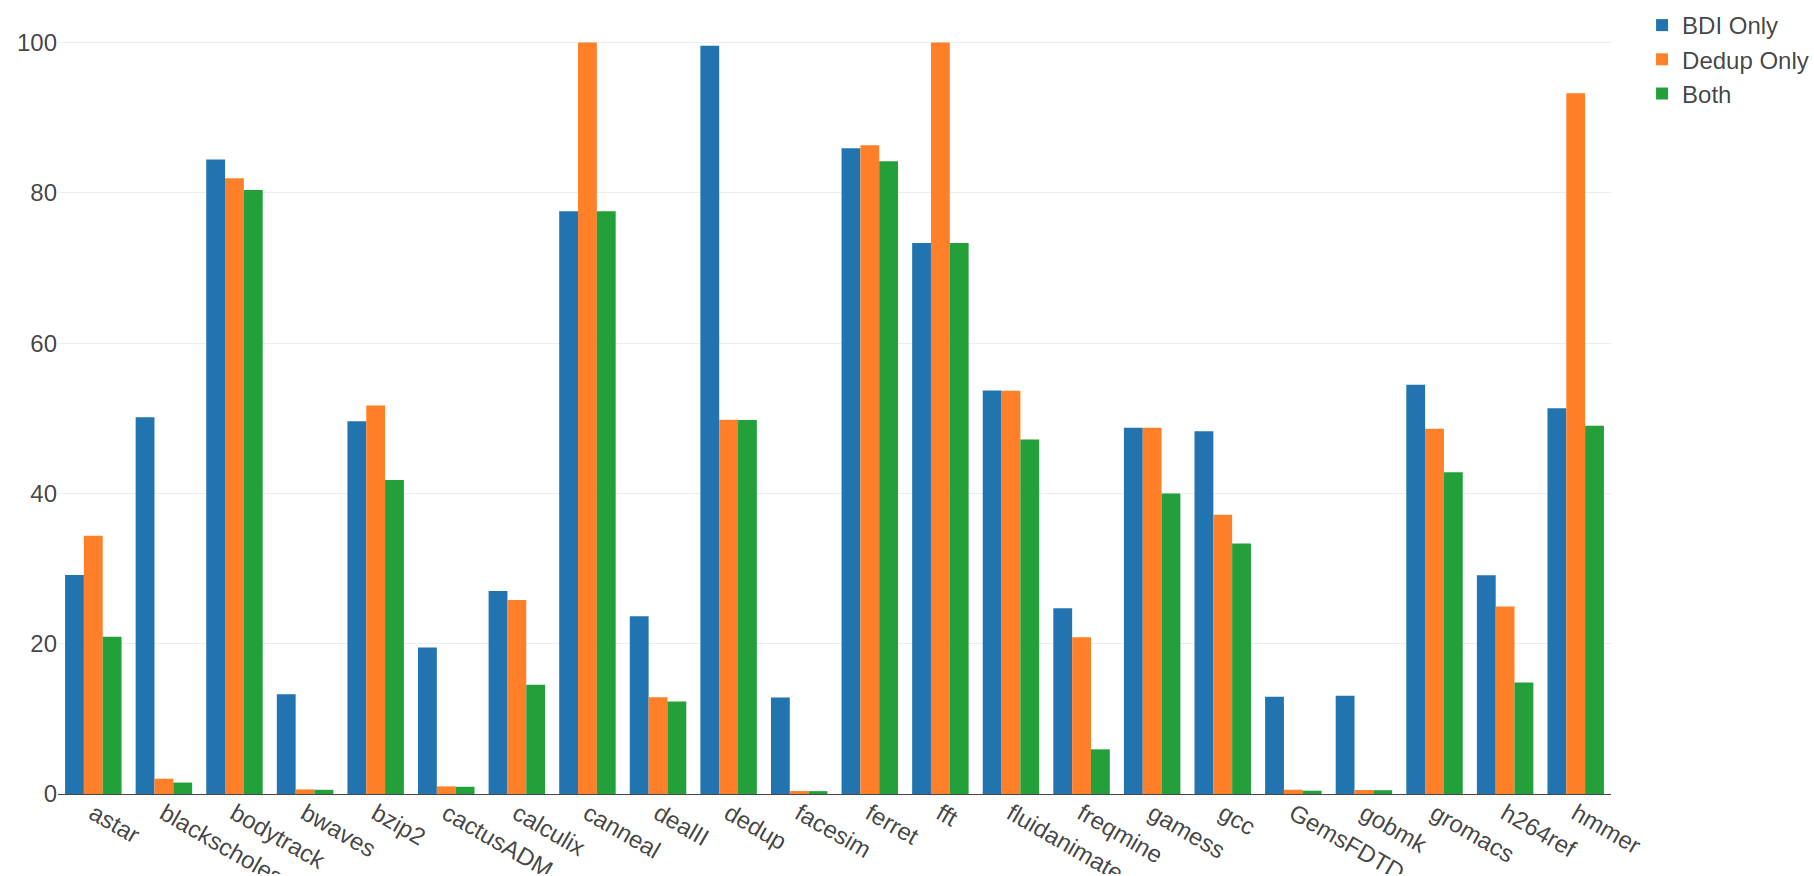
\includegraphics[width=\textwidth]{CompSize1.png}
    \end{subfigure}
    \begin{subfigure}[b]{\textwidth}
        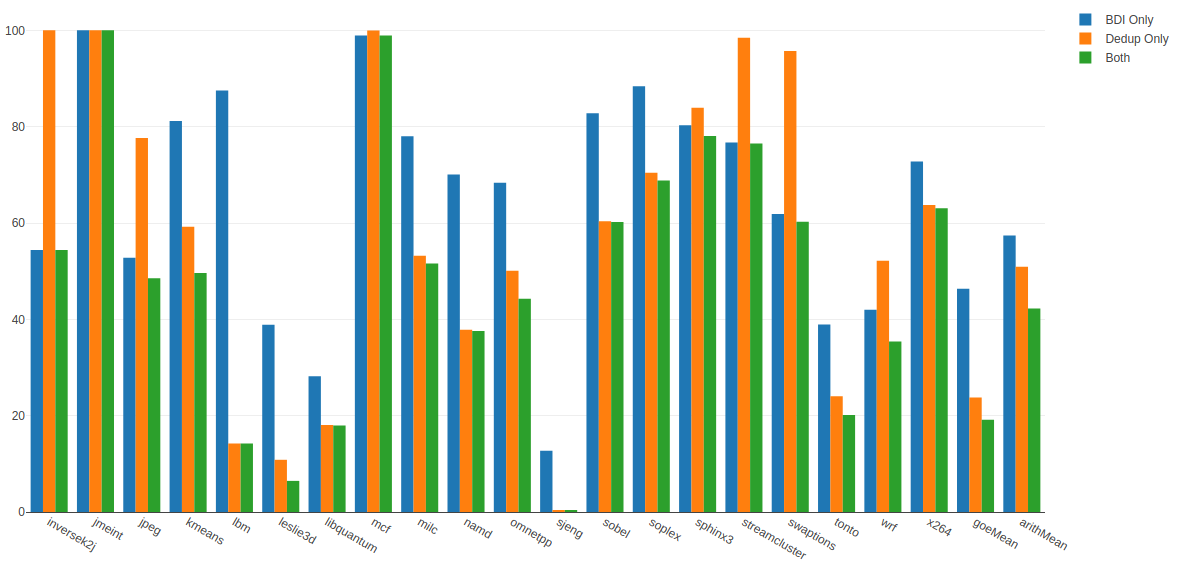
\includegraphics[width=\textwidth]{CompSize2.png}
    \end{subfigure}
    \caption[Size after compression]{The figure shows the size of data in a cache after using compression. BDI, Dedup, and a combination of both is shown.}
    \label{fig:CompSize}
\end{figure}
Nevertheless, combining BDI and Deduplication can still outperform each of them on its own. Figure~\ref{fig:CompSize} shows the compressed data size when using BDI, Dedup, and Dedup+BDI. In its worst case Dedup+BDI performs the same as the best out of Dedup and BDI, in most cases it compresses even more on both. Note that the experiments used to create Figure~\ref{fig:CompSize} are done statically on cache dumps and thus are completely missing the time dimension and its effect on compression. As time passes more requests to data lines can occur, with more requests the probability that compression can occur increases allowing for better compression.
